\documentclass[12pt,letterpaper]{article}
\usepackage[left=2.65cm,top=2.5cm,right=2.65cm,bottom=2.5cm]{geometry} 
\usepackage[english]{babel}
\usepackage[utf8x]{inputenc}
\usepackage{amsmath}
\usepackage{eqnarray}
\usepackage{mathtools}
\usepackage{amssymb} 
\usepackage[retainorgcmds]{IEEEtrantools}
\usepackage{booktabs,caption}
\usepackage[flushleft]{threeparttable}
\usepackage{graphicx}
\usepackage{tabularx}
\usepackage{subfig}
\usepackage{kpfonts}    % for nice fonts
\usepackage{microtype} 
\usepackage{booktabs}   % for nice tables
\usepackage{bm}         % for bold math
\usepackage{listings}   % for inserting code
\usepackage{verbatim}   % useful for program listings
\usepackage{color}  
%\usepackage[colorlinks=true]{hyperref}%%TABLE % use for hypertext
\usepackage[colorlinks = true,
            linkcolor = blue,
            urlcolor  = blue,
            citecolor = blue,
            anchorcolor = black]{hyperref}
\usepackage[colorinlistoftodos]{todonotes}
\usepackage{natbib}
\renewcommand{\baselinestretch}{1.25}



\begin{document}

%+Title
\title{\Huge{Market entry in the care homes sector\thanks{The authors are grateful for the comments received in WIPE workshop.}}}
\author{Eduardo Gonzalo Almorox\thanks{Newcastle University. Barrack Road} \thanks{Corresponding author: \tt{e.gonzalo-almorox@newcastle.ac.uk} } \and Nils Braakmaann\footnotemark[2]
 \and Volodymyr Bilotkchak\footnotemark[2] \and John Wildman\footnotemark[2]}


\date{First version: January 2016\\ This version: March 2016}
\maketitle

\begin{abstract}
This study investigates the effects of house prices in the English care homes market. 
High house prices, as experienced currently in England, may disincentive the entry in
 certain markets restricting the access to long term care services in these areas. Alternatively, 
 these areas may also suppose business opportunity. We provide evidence in order to disentangle 
 these effects. Our results suggest that higher house prices increase the rate care homes. 
 Based on unique dataset that collates information from several sources our analysis exploits 
 planning regulations to address empirical limitations associated with the house prices. Our findings
  contribute to inform policy makers about the relationship between the long term care and housing markets. 
\end{abstract}

{{\bf{Keywords}}: Care homes, house prices, long-term care, England\\
\bf{JEL}: R31, I12}

\newpage
\tableofcontents
%\newpage
%-Title


\newpage
\section{Introduction}
\label{sec: intro}

England has experienced the fastest growth in house prices amongst all OECD country during the last decades.
This inflationary trend has had consequences for both households, materialised in the so called “house affordability crisis”, 
and to less extent businesses. In this paper we investigate the relationship between the house prices 
and the market structure of an industry that typically operates with low margins, the care homes 
that provide long term care services. Our interest in the long term care is not trivial. Elements such as 
the ageing of the population or some socioeconomic changes that include the inclusion of more women 
in the labour force as well as the composition of different family structures, have shifted informal caregiving 
towards more formal long term care provision. These patterns evidence the importance of this sector in the 
forthcoming decades. Yet, despite the will of policy makers to design policies that preserve a sustainable 
provision of long term care and that also ensure competitive market structures, there is limited evidence for
 the design of these policies.  We aim at informing these policies by analysing the extent of the effect of high 
 prices in the housing market on the entries in the market of care homes. 

A major characteristic of the English market for long term care services consists of the geographical disparities
 in the levels of provision and funding and the consequent effects on other variables of interest for the market
 structure. \cite{forder2011} analysing data at local level, highlight the substantial differences in both 
 the level of need and the unit costs across English councils. This spatial variability seems to appear also in other
  variables of interest such as the levels of social care expenditure \citep{fernandez2015}. According 
  to these authors, a principal element to explain this local divergences are the underlying conditions that 
  providers face for supplying their services. Considering this, we argue that an element that may influence 
  the structure of the market for long term care services concerns the situation relative to the housing market. 
  Alike the former, the housing market in England also presents notable divergences across local areas that lead 
  to different levels of prices. Several authors have argued that this is a direct consequence of the different 
  designs associated with the planning regulations across the country. Hence, more restrictive planning 
  regulations result in higher levels of house prices (see for instance, \cite{cheshire2009} or \cite{hilber2016impact} for comprehensive reviews). 

The effect of house prices on the market entry of care homes is a priori uncertain. 
One possible explanation may consist of the influence of house prices as a cost for running a care home. 
Hence, high house prices may suppose an important barrier that can restrict the entry in certain markets.
 A potential consequence derived from the former, people living in these areas may find less long term care
  choices closer to them. A second argument may be on the basis of how high house prices may represent
   a business opportunity. The segment of the population that benefits from current upward trend in the house
    prices are those elderly homeowners that are able to monetize the higher value of their asset by selling their
     houses and moving out cheaper areas \citep{hilber2016housing}. If this argument holds, areas with higher 
     prices may be associated with greater levels of affluence and consequently greater proportions of clients
      that are more willing to pay for the services of a care home. Although the latter may contribute to preserve 
      the financial viability of care homes in the market, an issue that constitutes a current public policy concern, 
      it may also result in an unequal distribution of long term care across different areas in England where the
       most affluent areas are more benefited from a greater supply of home care services. 

In order to proceed with our analysis, we construct a unique dataset that merges information from several 
sources to collate information regarding the characteristics of the dynamics in the care homes market, the
 housing markets and the planning regulations. The dataset captures information regarding local authorities 
 at different level (e.g. street, district and county level). A first technical hurdle concerning the dataset, consists
  of distinguishing de novo entries associated with providers that effectively produce a new activity. Secondly, 
  there is an additional empirical caveat that we have to address with regards to effect of house price on care
   homes entries. It may be possible that care homes select markets that have high prices on a non-random 
   basis due to unobservable variables. This sample selection bias may invalidate the estimates corresponding
    to the effects of house prices. In order to overcome these, we carry out and identification strategy which 
    uses an instrumental variables approach that exploits the variability in the restrictiveness of planning
     regulations across English districts. Our identification relies on the assumption that changes in the planning
      requirements affect the entry of care homes in market through the levels of house prices. Our instrumental
       variables estimates indicate a positive relationship between the market entries and the house prices
        suggesting increases in the proportion of care homes of 0.21 when house prices increase by a 10\%.  
        We then can argue that higher house prices lead to greater market entries. These results suggest that
         providers would be focusing on areas where there are more expensive houses. 

To the best of our knowledge, no previous studies have been undertaken to provide causal evidence with
 regards to the effects of housing prices in the context of entries in the market of care homes. This research
  also makes a number of contributions to several strands of the literature. It provides further evidence to the 
  growing literature that analyses aspects associated with the market of care homes in England. \citet{forder2014} study the elements that determine the competition amongst care homes and assess the 
  consequences of this competition in both prices and quality. Also \citet{allan2015} evaluate empirically 
  the causes of market exits by investigating the effects of maintaining minimum standards in the quality of 
  the service. We extend this literature by addressing issues referred to the entry of care homes in the market. 
  Prior to this paper, only \cite{machin2003} have provided empirical evidence of factors affecting the market
   entry by analysing the effects of setting of a minimum wage. In addition to providing a more up to date
    evidence, this research uses a more extensive dataset provided by the regulator, the
     Care Quality Commission (CQC). Likewise, this research also extends the literature that studies the effects 
     of the planning system and the high house prices in England using the care homes as a new sector
      for the analysis. 

The rest of the paper is organised as follows. In the next section we introduce
 the institutional framework corresponding to the organisation of the local authorities
  responsible for planning activities and long term care. In Section 3 we outline the details
   associated with the sources of data and the variables used. Section 4 describes the empirical
    model and section 5 present the results. Finally, the main conclusions of the paper are shown in section 6. 

\section{Institutional background}
\label{sec: background}

In England planning and long term care are activities that are ruled and applied by local governments. 
The structure of these is nonetheless complex and entails different organizational levels\footnote{These levels or tiers include three main groups: (i) county councils, (ii) district, borough or city councils and (iii) parish or 
town councils. Most of the activities designed by local governments are developed at county or district level 
(group (i) or (ii))} depending on the type of services that are regulated. 
In this section we outline the main characteristics of the local government in England 
considering the particular cases of planning regulations and long term care. 
This will help to understand the geography that we adopting for our empirical analysis. 

\subsection{The English market for long term care}
\label{sec: long }

In England there are 152 local authorities that operate at council level\footnote{The Health and Social Care Act (2008) 
supposed the transfer of public health matters from Primary Care Trusts (PCT) 
to local authorities. Clinical issues were responsibility of the clinical commissioning groups (CCG).} and have 
responsibilities on long term care through the commissioning – e.g. purchase, of services.
 Since the mid-eighties, market mechanisms drive the provision of long term care services. 
 In this provision, the independent sector, which is composed by those providers whose services 
 are contracted by the NHS but their services are not owned or managed by the NHS, plays a major role. 
 Forder and Allan (2011), estimate that about a 90\% of the provision for older 
 people\footnote{Older people is the main group that compose the demand for long term care services. 
 However, care homes also provide services for other types of clients are young adults, people who have misused
 drugs.} was actually responsibility of the independent sector. Within this sector, the {\it for-profit} private 
 sector dominates the provision accumulating the majority of providers - about the 84\%.  
 
 There are various types of private providers depending on their size - e.g. the number of beds they have
  and their distribution is quite unbalanced. Jarrett (2016) argues that about the 15\% of market share is 
  concentrated in 4 “main providers” and the remaining 70\% of the market share is composed by providers 
  that have a reduced number of beds - no more than 0.4\% of the beds each. Despite this polarisation 
  within the private sector, the care homes market presents a high level of competitiveness overall. Alike
   the distribution of planning regulations, this competitiveness, is also subject to significant discrepancies 
   across different local authorities in England (Allan and Forder, 
   2012)\footnote{Considering registered care homes in all sectors, the South East is the region that has more registered care homes (currently more than 1,000). This proportion of care homes contrasts with the North East where there are about 360 registered care homes.}
 
 An underlying characteristic of the long term care market is associated with the types of demand that 
 providers face. In addition to publicly funded clients, who undertake a means test in order to determine 
 their eligibility for public support, there are also clients who self fund their care. Both types of clients
  purchase care distinctly and therefore are subject to two different market 
  configurations. Hence, 
  whereas self-funded clients purchase care normally according to market rules and their willingness
   to pay, the care of publicly funded clients is purchased through commissioners ultimately managed
    by the local authorities. The market for the latter adopts a form of quasi market where services obtain 
    a source of public funding from the state and/or local authorities but the provision is totally
     delivered by private and independent providers which compete for capturing those purchasers 
     that are publicly supported Le Grand, 2012\footnote{\bf{New paper on quasi markets}}. For the case of clients who receive public support, 
     there are several issues to consider regarding the way their care, and therefore their provider,
      is chosen. 

First, councils set a framework agreement where they establish their payment rates and their quality
 standards. These contracts are reviewed yearly considering the budgetary needs of the councils. 
 Providers willing to provide services according to the conditions in the agreement apply for inclusion.
  Once there is a list with potential providers that are prepared to charge fees based on the council
   payment rate, commissioners negotiate and choose amongst them. The main 
   driver of this choice is the fulfillment of the minimum quality standards. In some cases, local authorities
    carry out contracts in advance and block a number of places. Also, apart from allowing councils for
     acting on their behalf, clients who receive public support may choose personally their suitable
      accommodation among the locations included in the list. If the choice is not available, public clients 
      can choose an alternative location provided that the accommodation meets the needs of the client
       and the cost is not greater than the councils expected cost for people with the same degree of assessed needs.

The proportion of people supported publicly varies notably across different local authorities in England. 
Whereas local authorities located in the south east have a 44\% of the clients that are subsidized,
 other mostly located in the north east have almost an 80\% of clients that receive public support. This different
 degree of public support may lead to diverse market unbalances. In some cases. comissioners are the core clientele
 that care homes have and therefore negotiate contracts for a number of beds. This situation gives 
 them a purchasing power – monopsony - that leads to set prices below the equilibrium level.
  
The former situation entails distortions in both the demand and the supply side. 
The demand presents a cross-subsidisation of the services from the self-funded 
clients to the publicly-supported. Since providers offer the service with two 
different fees depending on who demands the service, {\it self-funded} clients 
must pay a premium to compenseate the discounts on the fees charged to public 
supported clients. Likewise, the supply side is also affected especially in the 
case of locations that rely notably on the clients that receive public support. In these cases, 
providers find greater hurdles to obtain enough margins to offset budgetary 
constraints. This situation may result in reductions on the
   quality of the services so that providers only meet the minimum standards required by the Care Quality
    Commission, reductions in the market entries or exits from the market (Allan and Forder, 2015)
    
  \subsection{Planning system in England}
  \label{sec: planning}
  
 Planning systems are responsibility of district councils throughout the local planning authorities. 
 These set out the strategic priorities for the areas throughout the Local Plans.
  These strategic priorities include the fulfilment of local needs at socio-economic, 
  cultural, security and health level. The former entail the intervention of other relevant agents
   in addition to the local planning authorities. In order to promote the engagement and a shared 
   decision making between both local planning authorities and other relevant parts since 2012 
   there is the National Planning Policy Framework. This is a framework that establishes a set of
    national planning policies in order to guide development decisions for meeting local needs. 
    The health and social care are issues explicitly addressed by the National Planning Framework.
     Concretely this framework must enhance the collaboration between local planning authorities, 
     public health authorities, commissioners and providers in order to promote healthy communities 
     and analyse the implications of the development of health and social care infrastructures. 
     The development of care homes constitutes then an element contained in the National Planning
      Framework. 
      
Several authors have investigated the effects associated with the design of the planning system in England 
and the net effects of the land use regulation. The main conclusions derived from this research are essentially
 two. Firstly, planning regulations in England are generally more restrictive than similar regulations in other
  countries such as for instance Germany (Cheshire 2013). As noted by Hilber (2011),
   various factors have contributed notably to restrict the housing supply. These have
    included the implementation of green belts, the controls in the height of the
     properties and the lack of fiscal incentives for the development at local level.
      In addition to those, local governments have a discretionary power to control
       the development of certain projects which is normally linked to political considerations
        and which increment the rigidities. The consequences of these rigid regulations have
         caused housing shortfalls \citep{cheshire2009, cheshire2014, hilber2016supply }
          and have translated into consistent increases in the house prices\footnote{See 
          see section~\ref{sec: results}
          for further details of the effects of tight planning regulations on house prices.} 
          Likewise, there has been a generalised up-ward trend in the volatility in the
           housing market (Cheshire (2013)). In any case, these analyses have not
            been focused just on the housing market. Conversely issues such as
             the losses of productivity in the retail sector (Cheshire et all, 2015)
              or the negative effects on small retailers derived from the creation
               of entry barriers to larger stores \cite{sadun2015}.  
               
               Secondly, the level of regulatory tightness differs notably across
                English local governments. Thus, local planning authorities
                 where there are more affluent areas (specially areas located in the South East England) 
                 tend to be more restrictive since they are subject to greater incentives to restrict 
                 the development and protect landlords and homeowners willing and therefore
                  exploit the likely increases the value of their assets. 
  

\section{Data and methods}
\label{sec: data}

  The data corresponding to  the sample of analysis in this paper cover years from 2011 to 2016 
  that we divide into three time intervals $t  (t = 1, 2, 3)$ that include March 2011 – March 2013, 
  March 2013 – March 2015 and March 2015 – September 2016. These data are 
  retrieved from several sources and are referreed to 324 local planning 
  authorities. We cluster our information at this level since these type of local authorities are likely to rule the housing planning policies and then 
  determine the house prices.  Therefore we assume that each of those represents a local market and
  a unit for the analysis. 
  
  \subsection*{Care homes}
  \label{sec: care homes}
  
  
 The information concerning the characteristics and dynamics of the
care homes is obtained from the Care Quality Commission (CQC) directory of active and inactive 
care homes. Our main interest consists of studying the effect of prices on the proportion of care homes 
in a local market. In the spirit of \citet{tokunaga2013factors}, who analyse
 the choice local markets by private long term care providers in Japan, we represent this proportion as the number
  of care homes per 1000 population in the local authority that
 are aged 65 or over. This dataset contains all the registrations of care homes that have carried out a regulated activity since
   2010. The initial sample includes 24,354 records. Our analysis is restricted to the entries from March
    2011 onwards since a substantive proportion of the total registrations (16,054) were 
     carried out during 2010 and the first two first months of 2011 as a result 
     of a new regulation.\footnote{Since October 2010 registration in Care Quality Commission  became a legal requirement for every long 
     term care provider who wanted to carry out a regulated activity.} As we illustrate in Figure \ref{fig: registrations}, this process 
     was prolonged for the remaining months of 2011 particularly until July. The forthcoming years presented  
     progressively a less intense level of registrations.
     
\begin{figure}[ht]
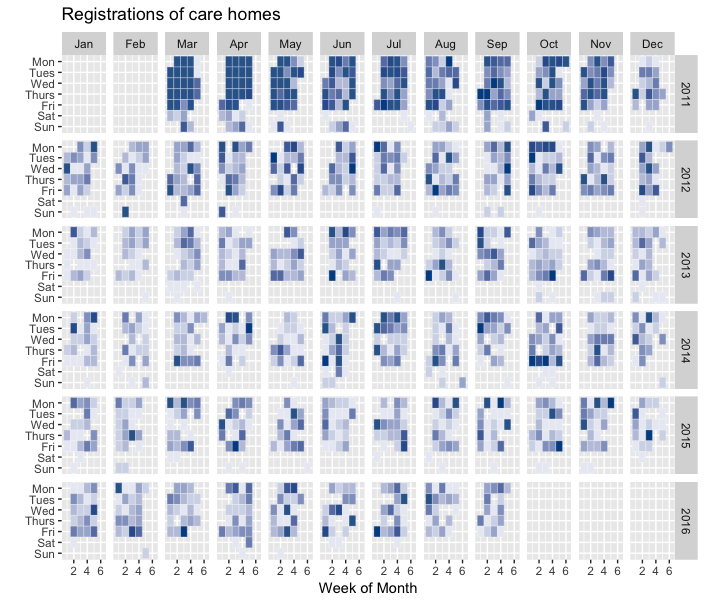
\includegraphics[width=1\textwidth]{registrations.png}
\caption{Care homes registrations in the CQC (2011- 2016)}
\label{fig: registrations}
\end{figure}


A major strength of this dataset for the purposes of this research consists of the opportunity to track the entries and exits of the care homes in the market. 
Concretely, this dataset records the date when each care home has been registered and deregistered (in case it has done so)
 in the CQC.  Besides, it provides further individual information regarding the care homes that includes 
the number of beds in the care home, the identifier code, the name of the care home, the postcode and postal 
address, the city and region where the care home is located as well as the local authority responsible for the 
social care activities corresponding to the location of the care home. Likewise, with the exception of the number of
 beds, the same information is available with regards to the providers where the care homes belong to. 
 We geocode all our observations in order to facilitiate the linkage with other 
 datasets.  Given that we do not have any further information available, we assume that care homes choose and stay in a market since the
       date of their registration. Analogously, we consider that a care home exits the market in the date that it is
        deregistered.

 
Considering the former, a general approach to calculate the proportion of care
 homes that are in the market consists of comparing the identification codes and dates
  of registration and deregistration. Then we can count the number of care homes that effectively 
  remain during each period of time. However, given the characteristics this administrative data from
   CQC it is necessary to stress an analytical caveat associated with the measurement of entries in the market.
    Concretely, it is important to differentiate those entries that correspond to {\it de novo entrants} –i.e. entries
     corresponding to firms that produce a new activity, from those that may be spurious referred to incumbent
      firms in the market and which are the result of change in the organizational structure or in the identification
       code. In our sample there are care homes that have been subject to modifications that include, changes
        in the address or take overs from a different provider. These changes are reflected in the registry with
         a change in the identification code. It is necessary to address these issues since neglecting them may
          hamper the results with regards to the market dynamics as well as bias subsequent conclusions at
           corporate level. \citet{geurts2016firm}, for instance, analyse the effect of this measurement
            problem on the estimations of the firm’s growth after the entry in the 
            market.\footnote{In the Appendix \ref{appendix market_entries} we present further details about the computation of this variable}
            
   

Likewise, in a second stage of our analysis we use information
corresponding to quality ratings. These are based on the system of inspections 
implemented by the CQC since 2014. On the basis of five 
dimensions\footnote{These dimensions entail the evaluation of issues related to the safety, the effectivity, 
the level of care and response to people’s needs as well as the management of the services.}, this new approach
  set a systematic method for collecting evidence that enables a more consistent assessment and comparison
   of the care homes’ performance. Services are rated according to four categories: {\it outstanding, good, requires
    improvement or inadequate}. For our analysis we collapse these categories into two: bad (requires improvement 
    and inadequate) and good (outstanding and good). Because the information is only available since October 2014, this part of the analysis considers a different
   timeframe that involves three waves from October 2014 - May 2015, May 2015 – February 2016 and 
   February 2016 – September 2016. 

\subsection*{House prices}
\label{sec: house prices}


   The information corresponding to prices of the properties is obtained from the price paid dataset
    released on a monthly basis by the Land Registry. This dataset contains all the transactions of
     properties carried out in England and Wales since 1995.  In addition to the price paid for the transaction,
    the dataset includes further information such as the type of property, the address, the city, district
     and region where the property is located as well as other information such as whether it is newly built
     and whether the property is under leasehold or freehold. The information regarding the transactions is
     collected on a daily basis we are able to subset the information according to the pre-defined periods of
     analysis. Then we group transactions that belong to the same planning authority and retrieve the average 
     price of them. The final output consists of an average price for each local planning authority for each
    period.  Prior to calculating the average prices, we geocode the transactions with the information of the postal code
    directory of the Office of National Statistics \cite{ons2016}.  We employ these
     geographical codes as key variables to match the information of house prices and the characteristics
      of the care homes. 
     
    
\subsection*{Instruments}

Inspired by \citet{hilber2016supply}, our identification strategy exploits the changes in the restrictiveness of the 
planning regulations. This variable is built considering a series of historical
  planning applications from the Department of Communities and Local Government (DCLG) 
  since 1978 and it is defined as the refusal of 10 dwellings or more per year. This variable is built considering
    information regarding planning applications from the Department of Communities and Local 
    Government (DCLG) and it is defined as the refusal of 10 dwellings or more per year. As we shall explain in further detail 
    below, this measure may be subject to endogeneity concerns. In order to correct for 
    these potential limitations, we use an alternative measure 
    of planning regulations, the rate in change of delay of major projects which is also obtained from the DCLG. We
    also use the variation in the historical 
    political composition of the local authorities. Using data from the British Election Studies Information System, 
    we capture a series of the historical Labour vote share at the General Election since 1983.
   




\subsection{Econometric framework}
\label{sec: specification}

Our purpose is to test the effect of the house prices on the proportion of care homes in local long term care markets.
Considering a local authority $i$ during a time period $t$, the proportion of care homes $C$ can be 
estimated with a simple regression model specified as follows
 
 \begin{eqnarray}
\label{eq: equation1}
   C_{it} = \beta X_{it} + \alpha P_{it} + \psi_{i} + \epsilon_{it}
 \end{eqnarray}

where $X_{it}$ represents a vector with different observable variables
 that characterize the composition of local long term care markets and that we use as controls. Hence, on the one hand
 we define the demand for long
  term care in the local market  by addressing a number of issues. Firstly, we include the proportion 
  of people older than 85 and proportion of people that receive the attendance 
  allowance\footnote{This benefit aims to support those people with physical disabilities in UK that live
   independently and might require residential care services otherwise. } as proxies of the level 
   of health dependency. Also, given the association between the financial needs and the funding
    support determined by the means-test, we incorporate the proportion of people that receive some
     sort of income support and the proportion of people that receive pension credits to reflect the payer 
     composition within the local population. These variables have been previously used in the literature for these purposes 
     \citep{darton2010slicing, forder2014}. Likewise, given that long term care is a labour intense activity,
      we add the proportion of females that claim for job seekers’ allowance in order to get a proxy for unemployment.  
      The information associated with this set of observable variables are 
      extracted from the Department of Work and Pensions. 
      
      In addition to the former, $X$ also includes a measure of the Herfindahl–Hirschman Index (HHI) to control for
      the competition between care homes in the local market. In our case, the HHI is a measure of concentration that 
      reflects the squared shares of beds across all the providers in a local market. The values range from
       0 to 1 where higher values represent higher concentration and therefore less competition. 
       
       
       
       $P_{it}$ is the average of the house prices and $\epsilon$
       represents an error term that is identically and independtly distributed. In this specification $\alpha$ is the 
       parameter of interest and thus is interpreted as the impact of house prices on the proportion 
       of care homes. Equation \ref{eq: equation1} can be estimated by OLS and will produce an unbiased estimate of $\alpha$ only if
         is exogenous so that $Cov(X_{i}, \epsilon_{i})$ . In case this occurs, this estimate may be effectively interpreted as
          a causal effect. 
          
 As we argue below, there may be elements that violate the former and introduce correlation between $P_{it}$ and
 $\epsilon_{it}$ resulting in biased estimates of $\alpha$. We address this concern by using an instrumental
  variables (IV) approach and estimating the two-least squares estimator of $\alpha$. We provide details of this
   strategy in the following subsection 
   
   \subsection{Bias and specification}
   
A potential element that can lead to inconsistent estimations of $\alpha$ may be the presence of unobserved
 variables that affect both house prices and proportion of care homes. For example, one may think about
  the effect of unobserved incomes that may affect positively the values of the properties and also incentivise
   the entries in the market given likely wealth effects. Hence, higher level of housing prices may result in
    wealth effects that lead to greater levels of consumption and then attract businesses. Hence the selection
     of an area by a care home provider is likely to be non-random and. In order to tackle with these potential
      problems, it is necessary to find an instrumental variable $z$  that is uncorrelated with $\epsilon$but is correlated
       with $P$
   
Our identification strategy for meeting this purpose is inspired on \citet{hilber2016supply}
The underlying idea of their strategy is based on exploiting the variability in the level of restrictiveness 
associated with planning regulations across UK planning authorities for analysing the effects of local earnings
 on house prices. Their findings confirm the vision that tight supply regimes – e.g. with more regulatory 
 constraints in the planning regulations, lead to increases in the prices. In our case, we apply directly 
 the planning regulation instruments to the house prices. For our identification we assume that this instrument,
  in addition of being correlated with local earnings as shown in 
  \citet{hilber2016supply}, is also correlated with the house prices. 
  
  Both the relationship between planning regulations and house prices as well as the use of planning regulations 
  for addressing endogeneity bias associated with house prices have been well documented in the literature. 
  Considering the case of UK, several authors have shed light with regards to the effects of tight planning 
  regulations on house prices suggesting a positive relationship
   (see for example \citet{bramley1998measuring, barker2004barker, hilber2016supply} Bramley (1998), Cheshire and Sheppard (1989, 2002), Barker (2004,2006), Cheshire and Hilber (2008) or Hilber and Vermeulen (2016)). 
The level of tightness of a local planning authority can be expressed in terms of the number of big “major”
 residential projects that are refused every year. 
    
    The results of Table 2 suggest that those local planning authorities that are more restrictive with the acceptance of 
    major project tend to have higher prices in their housing market. The use of the refusal rate could be considered
     as valid instrument for overcoming the endogeneity in house prices. However,
      as \citet{hilber2016supply} and \cite{hilber2015} argue, there some empirical concerns that have to be
       taken into account when using the refusal rates as instrument. First, this variable is pro-cyclical so 
       times with greater housing demand are linked to more regulatory restrictions. Thereby,
        the combination of these two elements may lead to greater increases of the house prices. 
        This problem can be addressed easily by using the average refusal rate. 
        
Yet there is a remaining problem concerning the way developers perceive the planning regulations. 
One may question whether the behaviour of developers is modified when they are aware of the level
 of tightness of certain local planning authorities are tighter than others. It may happen that if they know
  that some local planning authorities are particularly restrictive they may deter their applications and focus
   on other markets. If this occurs, then the observed refusal rates may not reflect the level of real 
   restrictiveness, especially in the cases of more limiting local planning authorities. For coping with this
    limitation it is possible to exploit two identification strategies on the basis of \cite{hilber2016supply}.
    
     The first involves a planning reform aimed at speeding up the planning processes and the
      second links the planning regulations and the variation in the share of local political power. 
The main idea corresponding to the identification strategy based on the planning reform consists
 of exploiting the variation in the change in the delay rates before and after the reform. Set in 2002,
  the reform included the establishment of an explicit goal for major development projects. The main
   purpose of this target was to avoid the delays of major projects by local planning authorities. Despite
    they were not formally penalised for not meeting the target, local planning authorities did not have
     the incentive for neglecting the target either. The central government could retain financial resources
      addressed to local planning authorities. An option for local authorities to meet the target was to refuse 
      greater projects and conversely approve smaller projects which could be finished on time. 
      
On the basis of the former, it is possible to think on the behaviour of the local planning authorities
 before and after the reform paying particular attention to their level of restrictiveness. Thus, before 
 the reform local planning authorities that were more restrictive would be also the ones that had greater 
 delays and thereby the least likely to meet the target. Once the reform was established, these local 
 planning authorities would be also the ones more likely to refuse more projects and therefore suffer less
  delays. Less restrictive local planning would not have to alter their behaviour substantially.
   Considering this, we allow for a 10-year period to represent the average delay rates pre and post reform.
    Hence we consider the delay rates 1994 and 1996 and the delay rates between 2004-2006.  
    
Regarding the relationship of political power and the application of local planning regulations we take
 advantage of the variation in the political composition of the local council. In addition to 
 \citet{hilber2016supply},
  this strategy has been used by other authors such \cite{bertrand2002does}, \cite{sadun2015} or Cheshire et al (2016).
  Hence, we use the share of Labour party votes at the General Election of 1983.
   The information is obtained from the British Election Studies Information System.  
   We choose the share of Labour voters since we believe that the attitudes of these voters 
   will be more inclined to grant house access rather than to preserve the value of the properties.
    Also, we could have used the results derived from local elections. 
    Yet, these might be correlated with the development of local housing markets and constitute a source
     of potential bias. The time frame of 1983 provides the earliest date where election results can be linked
      to data corresponding to local authorities and then minimizes the potential association between the
       outcome of the election and the planning process.
         
Considering these caveats, we specify \ref{eq: equation2} in order to estimate first-stage fitted values of the log
 house prices. The predicted values derived from this equation are used as instruments and incorporated in
 \ref{eq: equation1}in order to get a consistent estimate of $\alpha$.
 
  \begin{eqnarray}
\label{eq: equation2}
   P_{it} = \delta Z_{it} + X\kappa_{it} + u_{it}
 \end{eqnarray}

where $Z$ are a set of observables that will be used as instruments. 
For the reasons discussed above, we employ the share of Labour voters and the 
changes in delay rates pre and post reform.  $X$ incorporates the same set of market controls included in \ref{eq: equation1}.

\subsection{Descriptive statistics}

In Table 1 we summarise the main descriptive statistics for the variables of interest in our estimation sample. 
The information is presented at the level of local planning authorities and we also include the sources of 
information employed. On average, over the period of analysis (March 2013 – September 2016) 
there were about 1.7 care homes per 1000 population over 1000. Yet, this proportion varied notably 
across the different local planning authorities where some present less than 1 (0.4) care homes 
per 1000 population and some others more than 3.5 up to a maximum of 4.06. Other variables
 in Table 1 also reflect this local variation in the market for long term care. Interestingly there 
 is a planning authority that registers a maximum average value for the houses of £2,170,757. 
 Apart from this outlier, the average house prices are £267,014.
 
 As can be noted from Table 1, there are less observations associated with the information
  corresponding to the instrumental variables. This is because in 2010 there were certain
   Local Planning Authorities that were reformed and divided into new authorities.
    We are unable to retrieve and match the information corresponding to these new 
    authorities and therefore we drop then from the sample. In the next section we provide
  further details referred to the variables employed for our instrumental variables approach. 
  
  Furthermore, Figure 2 shows the geographical distribution of entries across 
  the local planning authorities considered in the analysis and provides
   further descriptive evidence that confirms the geographical differences with regards to entry and distribution
    of care homes in the long term care market. As can be noticed the highest entries tend to accumulate in the
     South east of and the local authorities around London. 

     Figure \ref{fig: house_prices} 
     plots the evolution on time the house prices across different regions in 
     England. 
     
     
\begin{figure}[h!]
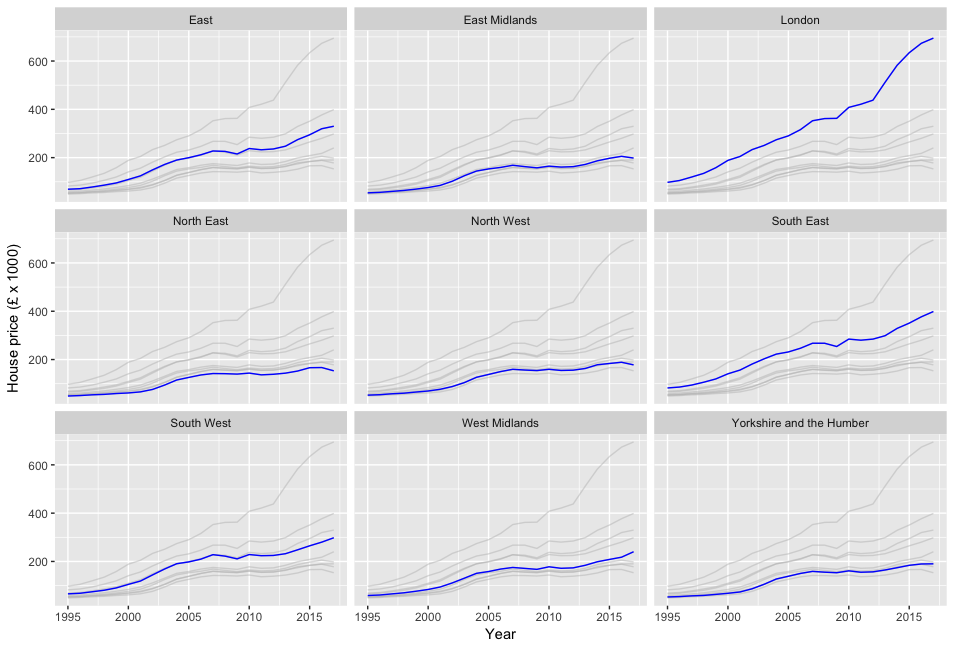
\includegraphics[width=1\textwidth]{house_prices_england.png}
\caption{House prices in England, 1995-2017}
\label{fig: house_prices}
\end{figure}
\label{sec:dependent variable}

\subsection{Prices and planning regulations}
Table 3 shows evidence on the validity of the instruments conidered. 
The two columns reflect estimates from regressions regarding \ref{eq: equation2 }with and without market 
controls respectively. If we consider the institutional mechanisms described in the former section, 
we we would expect that higher prices are associated also with tighter regulations. The results suggest 
a significant correlation between the house prices and all the instruments that we are proposing for both 
cases. The estimates also show the expected signs. Hence, the greater changes in the delay rates pre and
 post reform influence negatively the prices. Big differences imply reductions in the rate of delay for restrictive
  local authorities. These improvements are substituted with more rejections of the major projects and therefore 
  greater refusal rates. As we showed in Table 2 this variable is possitively associated with the house prices. 
  Likewise, the share of labour voters is also associated with lower levels in the house prices.

\begin{table}[h]
\centering
\caption{First stage results, dependent variable house prices (log)}
\label{table first_stage}
\resizebox{\textwidth}{!}{% 
\begin{tabular}{@{}llll@{}}
\toprule
                                    & Refusal rate & {Change rate of delay } & {Share votes of Labour} \\ 
\hline
House prices                        & 1.222***   & -0.095           & -1.672***          \\
                                    & (0.2802)     & (0.06)               & (0.328)              \\
\hline
Observations                        & 945          & 945                    & 945                   \\
R2                                  & 0.694        &                        &                       \\
Residual Std. Error                 & 0.279        &                        &                       \\
F Statistic                         & 52.25***     &                        &                       \\
\hline
Cragg-Donald Wald F statistic       &              & 4.56                   & 70.96                 \\
Kleibergen-Paap Wald rk F statistic &              & 2.07                   & 26.04                 \\ 
\bottomrule
\end{tabular}}
\begin{tablenotes}
      \scriptsize
      \item {\it{Notes}}: Market controls: Share of people 85+, 
      Share of people receiving Attendance Allowance, Share of people with pension credits, 
      Share of females claiming for Job Seekers Allowance, Share of adults with income support and
      Herfindahl-Hirschmann Index. Robust standard errors in parentheses. Standard errors are clustered at local planning 
      authority level. ***/**/*/$^{+}$ denote significance levels at 1\%, 5\%, 
      10\% and 15\%. Standard errors are presented in parentheses. 
    \end{tablenotes}
\end{table}


The results in table \ref{table first_stage}  show the predicted relationship between the house 
prices and the instruments proposed in \citep{hilber2016supply}. Prices in those planning authorities that are more 
restrictive and thus register higher refusal rates, present a positive 
association with house prices. Likewise, as \citet{hilber2016supply} indicate, 
the refusal rate may be subject to endogeneity concerns. 

This association is also reflected in figure 1 where we show further evidence on the validity of the instruments. 


\section{Results}
\label{sec: results}

\subsection{House prices and market entries}

Table 4 presents the main results derived from the estimation regarding the impact 
of house prices on the proportion of care homes based on the second stage of our 
specification in (1). The results in first three columns report the results associated
 with OLS estimates and indicate that the entries of care homes in the market are
  adversely affected by the level of prices in the housing market with the planning
   authority. This negative effect persists when we control for the observable 
   characteristics of the market and also control for county unobserved characteristics.
    Indeed, the greater impact of an increase of 10\% in the level of house prices leads to a decrease 
    of 0.035 in the number of care homes per 1000 population older than 65. This occurs when 
    we include both market and region controls in our estimation. When we only consider market
     controls a similar effect leads to a decrease of 0.019 care homes which is not significant. 
     The significant estimates when we include the county controls suggest that there may 
     be some unobserved variables that may bias the coefficient estimates regarding house prices. 

\begin{table}[ht]
\centering
\caption{Second stage results, effects of house prices on care homes entry}
\label{table second_stage}
\resizebox{\textwidth}{!}{% 
\begin{tabular}{@{}lllll@{}}
\toprule
                                    & \multicolumn{4}{c}{Care homes per 1000 people over 65}                                              \\ \midrule
                                    & \multicolumn{1}{c}{OLS} & \multicolumn{1}{c}{IV} & \multicolumn{1}{c}{OLS} & \multicolumn{1}{c}{IV} \\
\hline
Average house prices (log)                      & -0.111                  & 0.846*                &                         &                        \\
                                    & (0 .128 )              & (0.329)               &                         &                        \\
Average lagged house prices (log)             &                         &                        & -0.132            & 0.863**            \\
                                    &                         &                        & (0.127)                 & (0.33)               \\
\hline
Observations                        & 945                     & 945                    & 945                     & 945                    \\
R2                                  &                         & 0.1406                 &                         &                        \\
F statistic                         & 17.02***                &                        & 16.53***                &                        \\
\hline
Cragg-Donald Wald F statistic       &                         & 70.96                 &                         & 72.86                 \\
Kleibergen-Paap rk Wald F statistic &                         & 26.04                &                         & 29.12                 \\ 
\bottomrule
\end{tabular}}
\begin{tablenotes}
      \scriptsize
      \item {\it{Notes}}: Market controls: Share of people 85+, 
      Share of people receiving Attendance Allowance, Share of people with pension credits, 
      Share of females claiming for Job Seekers Allowance, Share of adults with income support and
      Herfindahl-Hirschmann Index. Robust standard errors in parentheses. Standard errors are clustered at local planning 
      authority level. ***/**/*/$^{+}$ denote significance levels at 1\%, 5\%, 
      10\% and 15\%. Standard errors are presented in parentheses. 
    \end{tablenotes}

\end{table}


The former estimates consider house prices as exogenous. However, as it has been discussed before, 
prices are subject to endogeneity concerns. Columns 4 to 9 show results where prices are treated as
 endogenous. Hence, columns 4 to 6 correspond to IV estimates incorporate the share of labour voters and columns
  7 – 9 include the changes in the rate of delay pre and post reform respectively. 
   As occurs with the OLS estimates, both IV regressions report results with and without 
   market and county level controls respectively. For assessing the validity and consistency of both instruments 
   we carry out Wald and Wu Hausman tests respectively. The results of these tests are displayed in the lower part
    of table \ref{table second_stage}. When we account for endogenity in our specifications, 
    the structure of the market for care homes seems to respond significantly to the differences in the local 
    housing markets. Nonetheless our results suggest now a different story with house prices affecting positively
     the entry of care homes given by proportion of care homes in the local market. Hence, the effect of house 
     prices on care homes entries shows a positive effect which generally is greater than the OLS estimates
      for the cases of market and country controls. The most important impact of a 10\% increase in the house
       prices corresponds to an increase of 0.21 in the number of care homes. This estimate, which is highly
        significant at lower level than 1\%, is obtained by using the share of labour voters as the instrument and 
        controlling for both market variables and county levels (column 6). Alternatively, when we control only for
         the market variable, we find that increases of 10\% in the house prices lead to significant increases of 0.11
          in the number of care homes. 
          
The Wald statistic indicates validity of the share of Labour voters as an instrument for the house prices in both
 the cases with and without controls. Likewise, the Wu-Hausman statistic suggests the rejection of the null 
 hypothesis of exogeneity in the house prices and therefore confirms the existence of endogeneity. Similarly,
  the rate of delay pre and post reform is also a valid instrument according to the Wald statistic when controlling 
  for market characteristics or neglecting controls. However, the estimates of the house prices instrumented by
   the rate of delay are less efficient than OLS estimates. The estimates of the Wu-Hausman estimates do not 
   allow to reject the exogeneity in the house prices.  
   
Also it is not possible to establish a clear conclusion regarding the effect of house prices
 given the results associated with the rates of delay pre and post-reform. Whereas this impact on the 
 proportion of care homes is positive when we control only for market variables, it turns to be negative 
 when we apply controls regarding region levels or no controls. Furthermore, in any of the cases these 
 effects are not significant. 
 
In general, these findings suggest that providers would be focusing on more affluent areas possibly 
aiming at securing potential clients that do not rely on public funding arrangements. A reason for
 this may be the aim of providers for minimizing the effect derived from the existing cross-subsidisation
  from self-funded to publicly funded clients. \cite{humphries2016social} argue that this strategy has been followed 
  by a number of long term care providers. 
  
 \subsubsection*{\normalsize{\it Robustness checks}}
 
In order to test the robustness of our results, we run various models.
 Firstly, a plausible concern may be the presence of some outliers in
  the distribution of care homes. In order to overcome the potential influence 
  of these observations we remove from the sample the top and bottom 5\% of care homes by 1000 population 
  over 65. We also consider a sample without the planning authorities belonging to the region of London.
   The results of these analyses are shown in Table 7. It is important to highlight that the specifications 
   corresponding to each of the columns are identical to the specifications presented in Table 
   \ref{table robustness}.
 
 
\begin{table}[h!]
\centering
\caption{Robustness checks, care homes without London region and  }
\label{table robustness}
\resizebox{\textwidth}{!}{% 
\begin{tabular}{@{}lllllllll@{}}
\toprule
                                    & \multicolumn{4}{c}{London excluded}        & \multicolumn{4}{c}{Top and bottom 5\% excluded}     \\ \midrule
                                    & OLS      & IV      & OLS       & IV        & OLS         & IV          & OLS       & IV          \\
\hline
House price                         & -0.21    & 1.612+ &           &           & 0.148** & 0.844** & 0.125 &             \\
                                    & (0.154)  & (0.998) &           &           & (0.075)     & (0.291)     & (0.076)   &             \\
Lagged house price                  &          &         & -0.206 & 1.473* &             &             &           & 0.857** \\
                                    &          &         & (0.150)   & (0.86)    &             &             &           & (0.29)      \\
\hline
Observations                        & 849      & 849     & 849       & 849       & 841         & 841         & 841       & 841         \\
R2                                  & 0.378    & 0.114   & 0.378     & 0.141     & 0.345       & 0.192       & 0.342     & 0.185       \\
F statistic                         & 15.31*** &         & 14.93***  & 11.43***  & 15.2***     & 11.69***    & 15.02***  & 12.03***    \\
\hline
Cragg-Donald Wald F statistic       &          & 25.207  &           & 28.677    &             & 74.324      &           & 77.821      \\
Kleibergen-Paap rk Wald F statistic &          & 11.156  &           & 13.887    &             & 22.603      &           & 25.896      \\ \bottomrule
\end{tabular}}

\begin{tablenotes}
      \scriptsize
      \item {\it{Notes}}: Market controls: Share of people 85+, 
      Share of people receiving Attendance Allowance, Share of people with pension credits, 
      Share of females claiming for Job Seekers Allowance, Share of adults with income support and
      Herfindahl-Hirschmann Index. Robust standard errors in parentheses. Standard errors are clustered at local planning 
      authority level. ***/**/*/$^{+}$ denote significance levels at 1\%, 5\%, 
      10\% and 15\%. Standard errors are presented in parentheses. 
    \end{tablenotes}

\end{table}


The results from Table \ref{table robustness}  are in general on the same lines 
as the results in Table \ref{table second_stage}. 

\subsection{Exploration of further channels}

\subsubsection*{\normalsize{\it Effect on the social care expenditure}}

The positive effect of prices  may be indicate a transfer of the demand. In Table \ref{table 4} 
we show the effect on the level of per capita expenditure in residential care. 

\begin{table}[h!]
\centering
\caption{Second stage results, effects on per capita expenditures}
\label{table 4}
\resizebox{\textwidth}{!}{% 
\begin{tabular}{@{}lllll@{}}
\toprule
                                    & \multicolumn{4}{c}{Per capita expenditure on residential care}                                      \\
                                    \hline
                                    & \multicolumn{1}{c}{OLS} & \multicolumn{1}{c}{IV} & \multicolumn{1}{c}{OLS} & \multicolumn{1}{c}{IV} \\
\hline
Average house prices (log)                        & -0.153                 & $-0.725 ^{+}$               &                         &                        \\
                                    & (0.122)               & (0.483)             &                         &                        \\
Average lagged house prices (log)                &                         &                        & -0.197                 & $-0.74 ^{+}$               \\
                                    &                         &                        & (0.128)               & (0.484 )            \\
\hline
Observations                        & 945                     & 945                    & 945                     & 945                    \\
R2                                  & 0.8604                  &                        &                         &                        \\
F statistic                         & 103.88***               &                        & 103.59***               &                        \\
\hline
Cragg-Donald Wald F statistic       &                         & 70.959                 &                         & 72.864                 \\
Kleibergen-Paap rk Wald F statistic &                         & 26.039                 &                         & 29.122              \\  
\bottomrule
\end{tabular}}
\begin{tablenotes}
      \scriptsize
      \item {\it{Notes}}: Market controls: Share of people 85+, 
      Share of people receiving Attendance Allowance, Share of people with pension credits, 
      Share of females claiming for Job Seekers Allowance, Share of adults with income support and
      Herfindahl-Hirschmann Index. Robust standard errors in parentheses. Standard errors are clustered at local planning 
      authority level. ***/**/*/$^{+}$ denote significance levels at 1\%, 5\%, 
      10\% and 15\%. Standard errors are presented in parentheses. 
    \end{tablenotes}

\end{table}

The effect of the prices in terms of the expenditure is how it would be 
expected. Higher houses reduce the levels of public expenditure on residential care.  
This effect is nonetheless very significant. An explanation may be derived from 
the fact that areas with higher prices may have less people that are likely to 
receive these funds. 



\subsubsection*{\normalsize{\it Effect on the distribution of care homes per level of quality}}

An alternative channel can be the distribution of care homes by their level of 
quality. In \ref{table quality} we show the resuls derived from the effect of house 
prices . We can see that the effects are to greater extent more pronounced in the case of care 
homes of better quality. In any case these effects are not significant.

\begin{table}[ht]
\centering
\caption{Second stage results, effects on distribution of care homes by quality}
\label{table quality}
\resizebox{\textwidth}{!}{% 
\begin{tabular}{@{}lcccccccc@{}}
\toprule
                                    & \multicolumn{4}{c}{Good quality care homes} & \multicolumn{4}{c}{Bad quality care homes} \\ \midrule
                                    & OLS           & IV          & OLS           & IV          & OLS           & IV          & OLS           & IV         \\
\hline
House prices                        & 0.144*       & 0.189       &               &             & 0.06**      & 0.02      &               &            \\
                                    & (0.086)       & (0.24)      &               &             & (0.018)        & (0.06)      &               &            \\
Lagged House prices                 &               &             & 0.138+       & 0.193      &               &             & 0.04*       & 0.02     \\
                                    &               &             & (0.09)        & (0.246)      &               &             & (0.02)        & (0.061)     \\
\hline
Observations                        & 945           & 945         & 945           & 945         & 945           &             & 945           &            \\
R2                                  & 0.2942        &             & 0.2936        &             & 0.4379        &             & 0.432         &            \\
F statistic                         & 12.34***      &             & 11.91***      &             & 21.25***      &             & 20.72***      &            \\
\hline
Cragg-Donald Wald F statistic       &               & 70.959      &               & 72.864      &               & 70.959      &               & 72.864     \\
Kleibergen-Paap rk Wald F statistic &               & 26.039      &               & 29.122      &               & 26.039      &               & 29.122     \\ \bottomrule
\end{tabular}}
\begin{tablenotes}
      \scriptsize
      \item {\it{Notes}}: Market controls: Share of people 85+, 
      Share of people receiving Attendance Allowance, Share of people with pension credits, 
      Share of females claiming for Job Seekers Allowance, Share of adults with income support and
      Herfindahl-Hirschmann Index. Robust standard errors in parentheses. Standard errors are clustered at local planning 
      authority level. ***/**/*/$^{+}$ denote significance levels at 1\%, 5\%, 
      10\% and 15\%. Standard errors are presented in parentheses. 
    \end{tablenotes}
\end{table}

When we control for endogeneity using the rate of delay as instrument for prices,
 contrary to the Labour share, the effects of the prices on the care homes entry
  are generally negative. The only significant effect 
  corresponds to the entry care homes classified as good and
   only when market controls are applied. It is also in this case,
    in addition to the case of no controls, when we should consider
     the delay rate as instrument for endogeneity. When we apply county controls. 


\section{Conclusion}

In this study we have investigated whether the high prices in the English housing market respresent a barrier to
 the provision of long term care services or contrarily they provide an incentive for care homes to set their 
 services. First, we test for simple OLS regression and we show that there are empirical constraints that produce
  biased estimates. Consequently we address these concerns by considering different variables associated with
    planning regulations to instrument the house prices. According to our findings, the use of the share of political
     power performs as a better instrument for addressing potential endogeneity concerns related to house prices.
       
       The results then suggest that house prices are positively associated with the entries and providers might
        therefore be driven to set their businesses in places where the prices of the properties higher. We explore 
        the underlying mechanism of this effect by examining how house prices affect the number of care 
        homes according to their quality rating. In sum, the positive effect of house prices on the entry of care
         homes is greater in cases where care homes have a better overall rating. A further avenue for this research
          could consider each of the dimensions involved in the quality inspections. 
          
Our results also point out at the connection between the housing market and the
 market of long term care activities. The coordination between local authorities at
  both county and district level is therefore encouraged to facilitate the provision of 
  further evidence about the relationships between both types of markets. 


\newpage
\bibliographystyle{apalike}
\bibliography{ex1}
%remember to use \citep{} for citation

\newpage
\section*{Appendix}

This appendix provides details on the various sources of data used as well as the computation of variables used in our empirical analysis. 

\subsection*{Market entries}
\label{appendix market_entries}

  For distinguishing de novo entries we firstly identify those postcodes that are repeated given that they may
      potentially contain spurious entries. Then, we compare the dates of registration, the identification code and
       the number of beds corresponding to each observation (care home) in order to identify those observations
        that effectively can be classified as a new entry in the market. Analogously, we follow a similar process for
         calculating the definite exits in the market.  Concretely, after casting those care homes with duplicated
          postcodes that report a date of deregistration\footnote{If the care home remains active,
           the observation corresponding to the date of deregistration is reported as missing.} 
           we compare identification codes and number of beds to define the last date as a definite exit. 
           Considering the former we can calculate the cumulative number of care homes for each wave
            and calculate the proportion of care homes for each 1000 inhabitants older than 65.   
\subsection{Geographical information}

 
  We attach several geographical information to the postcodes that we obtain from the postcode directory
   released by the Office of National Statistics \citep{ons2016}. Apart from arranging observations in terms of
    our unit of analysis, the local planning authorities, the underlying idea of incorporating this geographical
     information is to have a set of key variables that we can use for merging other data.         
     
     
\subsection*{Expenditures on social care} 

We extract this information from the different datsets available for creating the reports of Personal Social Services: Expenditure and Unit Costs, England. 
These reports are created on an annual basis and summarise the levels of expenditure on social care activities at council level. 
They are released by the NHS Digital\footnote{Further details may be found in \href{https://www.digital.nhs.uk/article/219/What-is-NHS-Digital-}{https://www.digital.nhs.uk/article/219/What-is-NHS-Digital-}} (formerly the HSCIC). 
For our analysis we select the information corresponding to the years 2011/12 - 2015/16. For representing the level
 of public expenditure we use the gross current expenditure. This is a well established fiscal measure of 
 government spending and it represents the expenditure that is not offset by income from clients and does not include capital charges either.\footnote{Gross current expenditure $G$
  is calculated as: $G = T - C$ where $T$ is Gross Total Expenditure and $C$ incorporates capital charges. 
  Likewise, $T$ is obtained from deducting incomes from joint arrangments $I$, the NHS $N$ and other incomes $O$ to the total expenditure
   $E$, $T = E - (I+N+O)$}

 In our analysis, we consider the spending devoted to residential care for indiviuals who were 65 or older. 
 The types of support on these individuals include physical support, sensory support, support with memory 
 and cognition, learning disability support and mental health support. 
 
 \subsection*{Election data}

We use two sources for obtaining the historical information corresponding
 to the British election results. The information that spans from 1983 to 2008
  us obtained from the British Center of Studies and is the information that we 
  use for our instrument. It aims at providing the historical profile of the electorate
   of the local authorities. Likewise we control for the rate of Labour voters from the last
    election available (June 2015). This information is obtained from the data
     platform\footnote{See \href{http://www.data.parliament.uk/dataset/general-election-2015} for further information}
\end{document}



